In this paper, we focus on the  Neyman-Pearson setting (see \cite{van1968detection}) where, given a test observation from (\ref{eq:stoch_setup}) or (\ref{eq:determ_setup}), a MSD is a likelihood ratio test (LRT) taking the form
\begin{equation}\label{eq:lrt}
\Lambda(y):=\dfrac{f(y|H_1)}{f(y|H_0)} \detgtrless \eta
\end{equation}
where $\Lambda(y)$ is the test statistic, $\eta$ is the threshold set to achieve a given false alarm rate, and $f$ is the appropriate conditional density of the test observation. \textcolor{blue}{In the following section, for both testing data models we derive the standard oracle detector (assuming all parameters are known) and plug-in detector (formed by substituting the parameter estimates of (\ref{eq:param_estims_stoch}) in the oracle detector). The oracle detectors, while unrealizable, give an upper bound for the performance of a MSD. We will see that when only finite training data is available (as is the case in real applications), the plug-in detector will realize a performance loss relative to this bound.}

\subsection{Stochastic Testing Model}\label{sec:plugin_stoch}
The LRT in (\ref{eq:lrt}) depends on the conditional distribution of the test vector, $y$. By properties of Gaussian random variables, when using the stochastic test model in (\ref{eq:stoch_setup}), these distributions are $y|H_0\sim\mathcal{N}\left(0,I_n\right)$ and $y|H_1\sim\mathcal{N}\left(0, U\Sigma U^H +I_n\right)$. The resulting LRT statistic is
\begin{equation}\label{eq:stoch_lrt}
\Lambda(y)=\frac{\mathcal{N}(0,U\Sigma U^H + I_n)}{\mathcal{N}(0,I_n)}.
\end{equation}
\textcolor{blue}{We derive an oracle detector by assuming that $k$, $\Sigma$, and $U$ are all known in (\ref{eq:stoch_lrt}). After simplification of this expression (see Section 4.14 of \cite{scharf1991statistical}), the oracle statistic becomes
\begin{equation}\label{eq:oracle_stat_stoch_y}
\Lambda_{\text{oracle}}(y) = y^HU\left(\Sigma^{-1}+I_k\right)^{-1}U^Hy.
\end{equation}
Note that the oracle statistic depends on the sufficient statistic $w:=U^Hy$. Using this notation, the oracle statistic is
\begin{equation}\label{eq:oracle_stat_stoch_w}
\boxed{\Lambda_{\text{oracle}}(w) = w^H\left(\Sigma^{-1}+I_k\right)^{-1}w = \sum_{i=1}^k\left(\frac{\sigma_i^2}{\sigma_i^2+1}\right)w_i^2}
\end{equation}
and the oracle detector is $\Lambda_{\text{oracle}}(w) \detgtrless \gamma_{\text{oracle}}$
%\begin{equation}\label{eq:oracle_class_stoch}
%\Lambda_{\text{oracle}}(w) \detgtrless \gamma_{\text{oracle}}
%\end{equation}
where the threshold $\gamma_{\text{oracle}}$ is chosen in the usual manner, \ie, so that it satisfies $P(\Lambda_{\text{oracle}}(w)>\gamma_{\text{oracle}}|H_0)=\alpha$ with $\alpha$ a desired false alarm rate. }

However, as the parameters $U$ and $\Sigma$ are unknown, the oracle statistic in (\ref{eq:oracle_stat_stoch_w}) cannot be computed. Given a dimension estimate $\widehat{k}$, we substitute the ML estimates of $U$ and $\Sigma$ given in (\ref{eq:param_estims_stoch}) for the unknown parameters in (\ref{eq:oracle_stat_stoch_y}) as similarly done in \cite{jin2005cfar} and \cite{mcwhorter2003matched}. \textcolor{blue}{This results in the plug-in detector's LRT statistic:} $
\Lambda_{\text{plugin}}(y)= y^H\widehat{U}\left(\widehat{\Sigma}^{-1}+I_{\widehat{k}}\right)^{-1}\widehat{U}^Hy$. Simplifying this expression using the statistic $\widehat{w} = \widehat{U}^Hy$, yields the plug-in statistic
\begin{equation}\label{eq:plugin_stat_stoch}
\boxed{\Lambda_{\text{plugin}}(\widehat{w}) = \widehat{w}^H\diag\left(\frac{\widehat{\sigma}^2_i}{\widehat{\sigma}^2_i+1}\right)\widehat{w}=\sum_{i=1}^{\widehat{k}}\left(\frac{\widehat{\sigma}_i^2}{\widehat{\sigma}_i^2+1}\right)\widehat{w}_i^2}
\end{equation}
and the plug-in detector takes the form $\Lambda_{\text{plugin}}(w) \detgtrless \gamma_{\text{plugin}}$
%\begin{equation}\label{eq:plugin_class_stoch}
%\Lambda_{\text{plugin}}(w) \detgtrless \gamma_{\text{plugin}}
%\end{equation}
where the threshold $\gamma_{\text{plugin}}$ is chosen in the usual manner.

The plug-in detector assumes that the estimated signal subspace, $\widehat{U}$, is equal to the true signal subspace, $U$, and that the estimated signal covariance, $\widehat{\Sigma}$, is equal to the true signal covariance, $\Sigma$. In other words,  the plug-in detector derivation assumes that $\widehat{U}^HU=I_{\widehat{k}}$, $\widehat{\sigma}_i^2=\sigma_i^2$ for $i=1,\dots,\widehat{k}$, and the provided subspace dimension estimate, $\widehat{k}$, is equal to the true underlying dimension of our signal subspace, $k$. Perhaps unsurprisingly, (as discussed in Section \ref{sec:rmt}) incorrectly choosing $\widehat{k}$ degrades the performance of the plug-in detector.

\subsection{Deterministic Testing Model}\label{sec:plugin_determ}
We now consider the alternative deterministic test vector model (\ref{eq:determ_setup}), which results in the following conditional distributions of the test vector $y|H_0\sim\mathcal{N}(0,I_n)$ and $y|H_1\sim\mathcal{N}(U\Sigma^{1/2} x, I_n)$. \textcolor{blue}{We begin by deriving an oracle detector, which assumes that $U$, $\Sigma$, $x$, and $k$ are all known. The LRT statistic for such a scenario is $\Lambda(y) = \frac{\mathcal{N}(U\Sigma^{1/2} x, I_n)}{\mathcal{N}(0,I_n)}$. Simplifying this expression leads to the oracle statistic
\begin{equation}\label{eq:determ_stat_oracle_y}
\Lambda_{\text{oracle}}(y) = x^H\Sigma^{1/2}U^Hy.
\end{equation}
As in the stochastic setting, $w=U^Hy$ is a sufficient statistic and the oracle statistic simplifies to
\begin{equation}\label{eq:determ_stat_oracle_w}
\boxed{\Lambda_{\text{oracle}}(w) = x^H\Sigma^{1/2}w = \sum_{i=1}^kx_i\sigma_iw_i.}
\end{equation}}

\textcolor{blue}{However, as the parameters $U$, $\Sigma$, and $x$  are unknown, the oracle statistic in (\ref{eq:determ_stat_oracle_w}) cannot be computed. Since we must estimate $x$ from the test vector, we employ the generalized likelihood ratio test (GLRT) where $\Lambda(y) = \frac{\max_x f(y|H_1)}{f(y|H_0)}$, resulting in the GLRT statistic
\begin{equation}\label{eq:glrt_determ}
\textcolor{blue}{\Lambda(y)=\frac{\max_x\mathcal{N}(U\Sigma^{1/2} x,I_n)}{\mathcal{N}(0,I_n)}.}
\end{equation}
Employing maximum likelihood estimation on $x$ in (\ref{eq:glrt_determ}) yields the estimate $\widehat{x}=\Sigma^{-1/2}U^Hy$.  Proceeding as in the stochastic setting, we substitute $\widehat{x}$ for the unknown $x$ in (\ref{eq:determ_stat_oracle_y}) and then substitute the ML estimates of $U$ and $\Sigma$ given in (\ref{eq:param_estims_stoch}) for the unknown $U$ and $\Sigma$ (see Section 4.11 of \cite{scharf1991statistical} for a similar treatment). This results in the plug-in statistic} $\Lambda_{\text{plugin}}(y) = y^H\widehat{U}\widehat{U}^Hy$. Again, $\widehat{w}=\widehat{U}^Hy$ is a statistic that can be used to write the plug-in statistic as
\begin{equation}\label{eq:plugin_stat_determ}
\boxed{\Lambda_{\text{plugin}}(\widehat{w}) = \widehat{w}^H\widehat{w}=\sum_{i=1}^{\widehat{k}}\widehat{w}_i^2},
\end{equation}
resulting in the detector $\Lambda_{\text{plugin}}(\widehat{w}) \detgtrless \gamma_{\text{plugin}}$, 
%\begin{equation}\label{eq:plugin_class_determ}
%\Lambda_{\text{plugin}}(\widehat{w}) \detgtrless \gamma_{\text{plugin}},
%\end{equation}
where the threshold $\gamma_{\text{plugin}}$ is chosen in the usual manner. \textcolor{blue}{The deterministic plug-in detector is an `energy detector', which sums the energy of the test observation lying in the subspace $\widehat{U}$.}

\subsection{Effect of the Number of Training Samples}\label{sec:training_effect}
\textcolor{blue}{In both the stochastic and deterministic testing settings, $\widehat{w}=\widehat{U}^Hy$ is a statistic used in the plug-in statistics (\ref{eq:plugin_stat_stoch}) and (\ref{eq:plugin_stat_determ}). This statistic relies on the estimated subspace $\widehat{U}$ formed from the top $\widehat{k}$ eigenvectors of the sample covariance matrix, $S$, of the training data. The stochastic detector also relies on the subpsace-SNR estimate $\widehat{\Sigma}$ formed from the top $\widehat{k}$ eigenvalues of $S$. For a fixed $\Sigma$, the accuracy of these estimates depends on the number of training data samples, $m$; we will mathematically show this in Section \ref{sec:rmt}. If we had access to an infinite amount of training data, the parameter estimates would be exact ($\widehat{U}\to U$ and $\widehat{\Sigma}\to\Sigma$). However, when we have access to only a finite amount of training data, $\widehat{U}$ and $\widehat{\Sigma}$ are inaccurate and will degrade the performance of the plug-in detectors with respect to the oracle detector, which provides an upper bound on detector performance.}

\begin{figure}[t]
\centering
\subfigure[Stochastic Setting]{
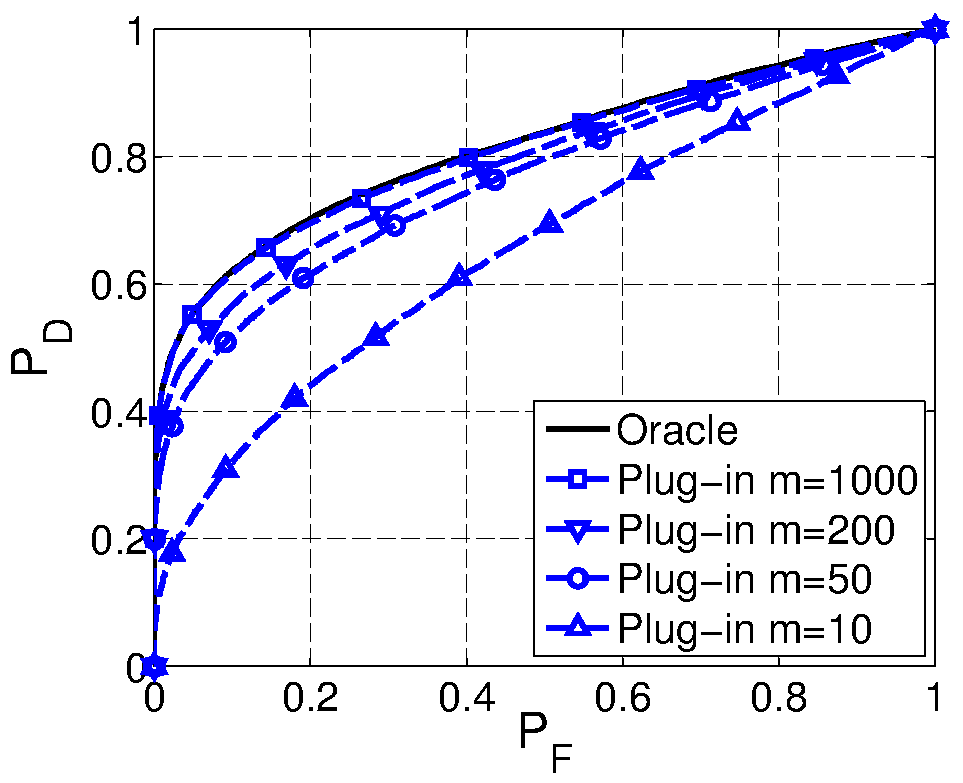
\includegraphics[width=1.5in]{figures/stoch_oracle_plugin.pdf}
\label{fig:stoch_oracle}
}
\subfigure[Deterministic Setting]{
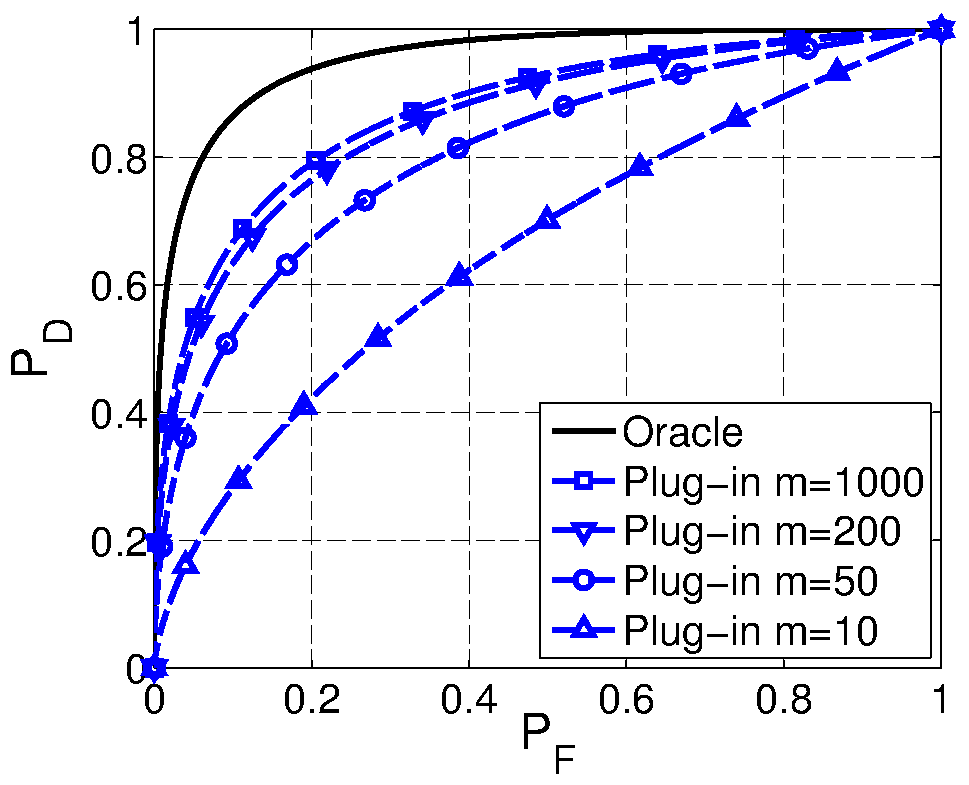
\includegraphics[width=1.5in]{figures/determ_oracle_plugin.pdf}
\label{fig:determ_oracle}
}
\vspace{-0.1in}
\caption{Empirical ROC curves for the plug-in and oracle detectors. Empirical ROC curves were simulated with $n=200$, $\widehat{k}=k=2$, and $\Sigma =\diag\left(10,0.1\right)$. The empirical ROC curves were computed using $10000$ test samples and averaged over 100 trials using algorithms 2 and 4 of \cite{fawcett2006introduction}. (a) Shows results for the stochastic MSD. (b) Shows results for the deterministic MSD when $x=[0.75,0.75]^T$. For both settings, as $m$ decreases, the performance of the plug-in detector degrades.}
\label{fig:plugin_v_oracle}
\vspace{-0.3in}
\end{figure}



\textcolor{blue}{To illustrate this performance loss, we consider a moderately sized system where $n=200$ and $\Sigma=\diag(10,0.1)$. We consider five detectors: the oracle detector and four plug-in detectors each using parameter estimates formed from varying amounts of training data. Figures \ref{fig:stoch_oracle} and \ref{fig:determ_oracle} plot the empirical ROC curves for the stochastic and deterministic testing settings, respectively. The amount of training data drastically affects the performance of the plug-in detector. As $m$ decreases, the plug-in detectors realize a significance performance loss. However, as $m\to\infty$, the plug-in detectors realize improved performance, closer to that of the oracle detectors.}

\textcolor{blue}{For the stochastic detector, as $m\to\infty$, the plug-in detector achieves the same performance as the oracle detector. Examination of the statistics (\ref{eq:oracle_stat_stoch_w}) and (\ref{eq:plugin_stat_stoch}) shows that these statistics will be identicial when $\widehat{U}\to U$ and $\widehat{\Sigma}\to\Sigma$, which is the case when infitie training data is available. However, this is not the case for the deterministic plug-in detector. Even with an infinite amount of training data, the plug-in detector will not achieve the oracle detector's performance. The deterministic plug-in detector must estimate $x$ given a noisy test observation $y$, which is independent from the training data. Even with infinite training data causing $\widehat{U}\to U$ and $\widehat{\Sigma}\to\Sigma$, $\widehat{x}$ does not converge to $x$. Therefore, the deterministic plug-in detector cannot achieve the performance bound of the oracle detector, which assumes that $x$ is known.}

\textcolor{blue}{For a fixed probability of false alarm ($P_F$), we can explore this performance loss by comparing the achieved probability of detection ($P_D$) of the plug-in detector to that of the oracle detector. Let
\begin{equation}\label{eq:epsilon}
\epsilon = 1 - \frac{P_D^{\text{plugin}}}{P_D^{\text{oracle}}}
\end{equation}
be the performance loss of the plug-in detector. Figure \ref{fig:epsilon_graph} empirically plots the number of training samples needed to achieve a desired performance loss $\epsilon$ for the stochastic plug-in detector. There is an exponential relationship between $\epsilon$ and $m$ indicating that we need infinite training samples to achieve zero performance loss ($\epsilon=0$). However, in any practical application we will never have an infinite amount of training data and so the plug-in detector will realize some non-zero performance loss. The rest of the paper will mathematically predict how finite training data affects detector performance and will derive new detectors to avoid some of this performance loss.}

\begin{figure}[t]
\centering
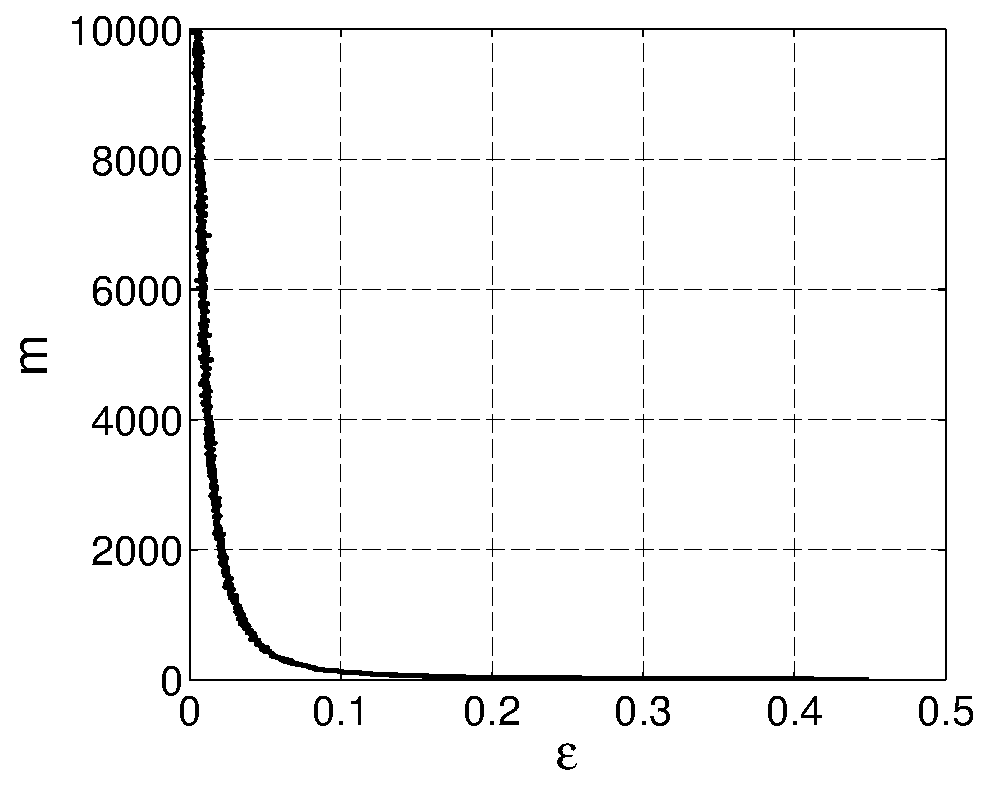
\includegraphics[width=1.5in]{figures/epsilon_graph.pdf}
\vspace{-0.1in}
\caption{Empirically determined number of training samples, $m$,  needed for the stochastic plug-in detector to achieve a desired performance loss, $\epsilon$, as defined in (\ref{eq:epsilon}). The required false alarm rate is $P_F=0.1$. Emprical ROC curves were generated for $n=200$, $\Sigma=\diag(10,0.1)$, $\widehat{k}=k=2$ using 10000 testing samples and averaged over 100 trials using algorithms 2 and 4 of \cite{fawcett2006introduction}.}
\label{fig:epsilon_graph}
\vspace{-0.3in}
\end{figure}
